\documentclass[twoside]{book}

% Packages required by doxygen
\usepackage{fixltx2e}
\usepackage{calc}
\usepackage{doxygen}
\usepackage[export]{adjustbox} % also loads graphicx
\usepackage{graphicx}
\usepackage[utf8]{inputenc}
\usepackage{makeidx}
\usepackage{multicol}
\usepackage{multirow}
\PassOptionsToPackage{warn}{textcomp}
\usepackage{textcomp}
\usepackage[nointegrals]{wasysym}
\usepackage[table]{xcolor}

% Font selection
\usepackage[T1]{fontenc}
\usepackage[scaled=.90]{helvet}
\usepackage{courier}
\usepackage{amssymb}
\usepackage{sectsty}
\renewcommand{\familydefault}{\sfdefault}
\allsectionsfont{%
  \fontseries{bc}\selectfont%
  \color{darkgray}%
}
\renewcommand{\DoxyLabelFont}{%
  \fontseries{bc}\selectfont%
  \color{darkgray}%
}
\newcommand{\+}{\discretionary{\mbox{\scriptsize$\hookleftarrow$}}{}{}}

% Page & text layout
\usepackage{geometry}
\geometry{%
  a4paper,%
  top=2.5cm,%
  bottom=2.5cm,%
  left=2.5cm,%
  right=2.5cm%
}
\tolerance=750
\hfuzz=15pt
\hbadness=750
\setlength{\emergencystretch}{15pt}
\setlength{\parindent}{0cm}
\setlength{\parskip}{3ex plus 2ex minus 2ex}
\makeatletter
\renewcommand{\paragraph}{%
  \@startsection{paragraph}{4}{0ex}{-1.0ex}{1.0ex}{%
    \normalfont\normalsize\bfseries\SS@parafont%
  }%
}
\renewcommand{\subparagraph}{%
  \@startsection{subparagraph}{5}{0ex}{-1.0ex}{1.0ex}{%
    \normalfont\normalsize\bfseries\SS@subparafont%
  }%
}
\makeatother

% Headers & footers
\usepackage{fancyhdr}
\pagestyle{fancyplain}
\fancyhead[LE]{\fancyplain{}{\bfseries\thepage}}
\fancyhead[CE]{\fancyplain{}{}}
\fancyhead[RE]{\fancyplain{}{\bfseries\leftmark}}
\fancyhead[LO]{\fancyplain{}{\bfseries\rightmark}}
\fancyhead[CO]{\fancyplain{}{}}
\fancyhead[RO]{\fancyplain{}{\bfseries\thepage}}
\fancyfoot[LE]{\fancyplain{}{}}
\fancyfoot[CE]{\fancyplain{}{}}
\fancyfoot[RE]{\fancyplain{}{\bfseries\scriptsize Generated by Doxygen }}
\fancyfoot[LO]{\fancyplain{}{\bfseries\scriptsize Generated by Doxygen }}
\fancyfoot[CO]{\fancyplain{}{}}
\fancyfoot[RO]{\fancyplain{}{}}
\renewcommand{\footrulewidth}{0.4pt}
\renewcommand{\chaptermark}[1]{%
  \markboth{#1}{}%
}
\renewcommand{\sectionmark}[1]{%
  \markright{\thesection\ #1}%
}

% Indices & bibliography
\usepackage{natbib}
\usepackage[titles]{tocloft}
\setcounter{tocdepth}{3}
\setcounter{secnumdepth}{5}
\makeindex

% Hyperlinks (required, but should be loaded last)
\usepackage{ifpdf}
\ifpdf
  \usepackage[pdftex,pagebackref=true]{hyperref}
\else
  \usepackage[ps2pdf,pagebackref=true]{hyperref}
\fi
\hypersetup{%
  colorlinks=true,%
  linkcolor=blue,%
  citecolor=blue,%
  unicode%
}

% Custom commands
\newcommand{\clearemptydoublepage}{%
  \newpage{\pagestyle{empty}\cleardoublepage}%
}

\usepackage{caption}
\captionsetup{labelsep=space,justification=centering,font={bf},singlelinecheck=off,skip=4pt,position=top}

%===== C O N T E N T S =====

\begin{document}

% Titlepage & ToC
\hypersetup{pageanchor=false,
             bookmarksnumbered=true,
             pdfencoding=unicode
            }
\pagenumbering{alph}
\begin{titlepage}
\vspace*{7cm}
\begin{center}%
{\Large 162lib }\\
\vspace*{1cm}
{\large Generated by Doxygen 1.8.13}\\
\end{center}
\end{titlepage}
\clearemptydoublepage
\pagenumbering{roman}
\tableofcontents
\clearemptydoublepage
\pagenumbering{arabic}
\hypersetup{pageanchor=true}

%--- Begin generated contents ---
\chapter{Class Index}
\section{Class List}
Here are the classes, structs, unions and interfaces with brief descriptions\+:\begin{DoxyCompactList}
\item\contentsline{section}{\hyperlink{structtData}{t\+Data} \\*C/\+C++ library I use for some programs, which includes exercises done at school }{\pageref{structtData}}{}
\end{DoxyCompactList}

\chapter{File Index}
\section{File List}
Here is a list of all documented files with brief descriptions\+:\begin{DoxyCompactList}
\item\contentsline{section}{src/\hyperlink{162lib_8c}{162lib.\+c} }{\pageref{162lib_8c}}{}
\item\contentsline{section}{src/{\bfseries 162lib.\+h} }{\pageref{162lib_8h}}{}
\end{DoxyCompactList}

\chapter{Class Documentation}
\hypertarget{structtData}{}\section{t\+Data Struct Reference}
\label{structtData}\index{t\+Data@{t\+Data}}


C/\+C++ library I use for some programs, which includes exercises done at school.  




{\ttfamily \#include $<$162lib.\+h$>$}

\subsection*{Public Attributes}
\begin{DoxyCompactItemize}
\item 
int \hyperlink{structtData_a71d1e2d3a39ed332ae5fbe49047e92fb}{day}
\item 
int \hyperlink{structtData_a09255da5529c4457e9bac181f6ebabac}{month}
\item 
int \hyperlink{structtData_abc54df4b847929f10f39352918fe0e0f}{year}
\end{DoxyCompactItemize}


\subsection{Detailed Description}
C/\+C++ library I use for some programs, which includes exercises done at school. 

\begin{DoxyAuthor}{Author}
Lorenzo \char`\"{}lorecast162\char`\"{} Cauli 
\end{DoxyAuthor}
\begin{DoxyDate}{Date}
September 2019 Struct used for date storage 
\end{DoxyDate}


Definition at line 12 of file 162lib.\+h.



\subsection{Member Data Documentation}
\mbox{\Hypertarget{structtData_a71d1e2d3a39ed332ae5fbe49047e92fb}\label{structtData_a71d1e2d3a39ed332ae5fbe49047e92fb}} 
\index{t\+Data@{t\+Data}!day@{day}}
\index{day@{day}!t\+Data@{t\+Data}}
\subsubsection{\texorpdfstring{day}{day}}
{\footnotesize\ttfamily int t\+Data\+::day}

Day field 

Definition at line 14 of file 162lib.\+h.



Referenced by data\+Read(), and fdata\+Read().

\mbox{\Hypertarget{structtData_a09255da5529c4457e9bac181f6ebabac}\label{structtData_a09255da5529c4457e9bac181f6ebabac}} 
\index{t\+Data@{t\+Data}!month@{month}}
\index{month@{month}!t\+Data@{t\+Data}}
\subsubsection{\texorpdfstring{month}{month}}
{\footnotesize\ttfamily int t\+Data\+::month}

Month field 

Definition at line 16 of file 162lib.\+h.



Referenced by data\+Read(), and fdata\+Read().

\mbox{\Hypertarget{structtData_abc54df4b847929f10f39352918fe0e0f}\label{structtData_abc54df4b847929f10f39352918fe0e0f}} 
\index{t\+Data@{t\+Data}!year@{year}}
\index{year@{year}!t\+Data@{t\+Data}}
\subsubsection{\texorpdfstring{year}{year}}
{\footnotesize\ttfamily int t\+Data\+::year}

Year field 

Definition at line 18 of file 162lib.\+h.



Referenced by data\+Read(), and fdata\+Read().



The documentation for this struct was generated from the following file\+:\begin{DoxyCompactItemize}
\item 
src/162lib.\+h\end{DoxyCompactItemize}

\chapter{File Documentation}
\hypertarget{162lib_8c}{}\section{src/162lib.c File Reference}
\label{162lib_8c}\index{src/162lib.\+c@{src/162lib.\+c}}
{\ttfamily \#include \char`\"{}162lib.\+h\char`\"{}}\newline
{\ttfamily \#include $<$stdio.\+h$>$}\newline
{\ttfamily \#include $<$stdlib.\+h$>$}\newline
{\ttfamily \#include $<$time.\+h$>$}\newline
Include dependency graph for 162lib.c\+:\nopagebreak
\begin{figure}[H]
\begin{center}
\leavevmode
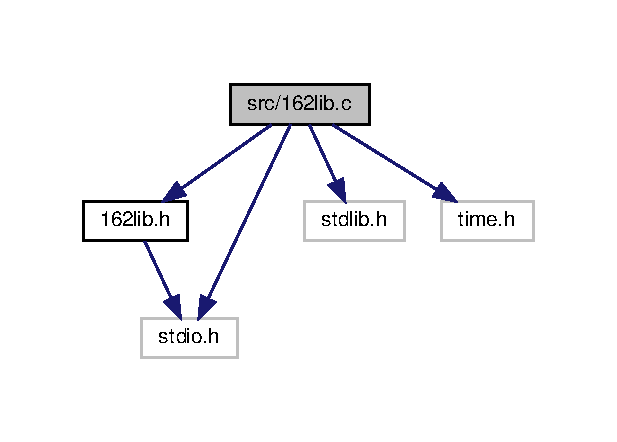
\includegraphics[width=296pt]{162lib_8c__incl}
\end{center}
\end{figure}
\subsection*{Functions}
\begin{DoxyCompactItemize}
\item 
F\+I\+LE $\ast$ \hyperlink{162lib_8c_a840caba325fc39fa2e29144229b66a8a}{file\+Open} (const char filename\mbox{[}$\,$\mbox{]}, const char perm\mbox{[}$\,$\mbox{]})
\item 
void \hyperlink{162lib_8c_aab64c14e0c8d540650ac483c451ace85}{data\+Read} (\hyperlink{structtData}{t\+Data} out)
\item 
void \hyperlink{162lib_8c_a5f08457e89eab8c32d89799c8c647054}{fdata\+Read} (F\+I\+LE $\ast$file, \hyperlink{structtData}{t\+Data} out)
\item 
void \hyperlink{162lib_8c_a44edab2dbf74abe9e90db151e1915fb1}{rnd\+Gen\+Init} ()
\item 
int \hyperlink{162lib_8c_a96cf9e2f003ddc8af7d221d7287edb75}{rnd} (int min, int max)
\end{DoxyCompactItemize}


\subsection{Detailed Description}
This is where the code for the library resides. 

\subsection{Function Documentation}
\mbox{\Hypertarget{162lib_8c_aab64c14e0c8d540650ac483c451ace85}\label{162lib_8c_aab64c14e0c8d540650ac483c451ace85}} 
\index{162lib.\+c@{162lib.\+c}!data\+Read@{data\+Read}}
\index{data\+Read@{data\+Read}!162lib.\+c@{162lib.\+c}}
\subsubsection{\texorpdfstring{data\+Read()}{dataRead()}}
{\footnotesize\ttfamily void data\+Read (\begin{DoxyParamCaption}\item[{\hyperlink{structtData}{t\+Data}}]{out }\end{DoxyParamCaption})}

Read date in a format to be stored in a struct of type \hyperlink{structtData}{t\+Data} with stdin as input stream.


\begin{DoxyParams}{Parameters}
{\em out} & The record into which the date needs to be stored. \\
\hline
\end{DoxyParams}


Definition at line 20 of file 162lib.\+c.



References t\+Data\+::day, t\+Data\+::month, and t\+Data\+::year.


\begin{DoxyCode}
20                         \{
21     scanf(\textcolor{stringliteral}{"%d%*c"}, &out.\hyperlink{structtData_a71d1e2d3a39ed332ae5fbe49047e92fb}{day});
22     scanf(\textcolor{stringliteral}{"%d%*c"}, &out.\hyperlink{structtData_a09255da5529c4457e9bac181f6ebabac}{month});
23     scanf(\textcolor{stringliteral}{"%d%*c"}, &out.\hyperlink{structtData_abc54df4b847929f10f39352918fe0e0f}{year});
24 \}
\end{DoxyCode}
\mbox{\Hypertarget{162lib_8c_a5f08457e89eab8c32d89799c8c647054}\label{162lib_8c_a5f08457e89eab8c32d89799c8c647054}} 
\index{162lib.\+c@{162lib.\+c}!fdata\+Read@{fdata\+Read}}
\index{fdata\+Read@{fdata\+Read}!162lib.\+c@{162lib.\+c}}
\subsubsection{\texorpdfstring{fdata\+Read()}{fdataRead()}}
{\footnotesize\ttfamily void fdata\+Read (\begin{DoxyParamCaption}\item[{F\+I\+LE $\ast$}]{file,  }\item[{\hyperlink{structtData}{t\+Data}}]{out }\end{DoxyParamCaption})}

Read date in a format to be stored in a struct of type \hyperlink{structtData}{t\+Data} with file as input stream.


\begin{DoxyParams}{Parameters}
{\em file} & Pointer to the file from which the function will read. \\
\hline
{\em out} & The record into which the date needs to be stored. \\
\hline
\end{DoxyParams}


Definition at line 26 of file 162lib.\+c.



References t\+Data\+::day, t\+Data\+::month, and t\+Data\+::year.


\begin{DoxyCode}
26                                      \{
27     fscanf(file, \textcolor{stringliteral}{"%d%*c"}, &out.\hyperlink{structtData_a71d1e2d3a39ed332ae5fbe49047e92fb}{day});
28     fscanf(file, \textcolor{stringliteral}{"%d%*c"}, &out.\hyperlink{structtData_a09255da5529c4457e9bac181f6ebabac}{month});
29     fscanf(file, \textcolor{stringliteral}{"%d%*c"}, &out.\hyperlink{structtData_abc54df4b847929f10f39352918fe0e0f}{year});
30 \}
\end{DoxyCode}
\mbox{\Hypertarget{162lib_8c_a840caba325fc39fa2e29144229b66a8a}\label{162lib_8c_a840caba325fc39fa2e29144229b66a8a}} 
\index{162lib.\+c@{162lib.\+c}!file\+Open@{file\+Open}}
\index{file\+Open@{file\+Open}!162lib.\+c@{162lib.\+c}}
\subsubsection{\texorpdfstring{file\+Open()}{fileOpen()}}
{\footnotesize\ttfamily F\+I\+LE$\ast$ file\+Open (\begin{DoxyParamCaption}\item[{const char}]{filename\mbox{[}$\,$\mbox{]},  }\item[{const char}]{perm\mbox{[}$\,$\mbox{]} }\end{DoxyParamCaption})}

Open a file given path and mode.


\begin{DoxyParams}{Parameters}
{\em filename} & File path passed as a string. \\
\hline
{\em perm} & File open mode passed as a string.\\
\hline
\end{DoxyParams}
\begin{DoxyReturn}{Returns}
Pointer to opened file\textquotesingle{}s I/O stream. 
\end{DoxyReturn}


Definition at line 10 of file 162lib.\+c.


\begin{DoxyCode}
10                                                         \{
11         FILE* out;
12         out = fopen(filename, perm);
13         \textcolor{keywordflow}{if} (out == NULL)\{
14                 perror(\textcolor{stringliteral}{"File opening error.\(\backslash\)n"});
15                 exit(-1);
16         \}
17         \textcolor{keywordflow}{return} out;
18 \}
\end{DoxyCode}
\mbox{\Hypertarget{162lib_8c_a96cf9e2f003ddc8af7d221d7287edb75}\label{162lib_8c_a96cf9e2f003ddc8af7d221d7287edb75}} 
\index{162lib.\+c@{162lib.\+c}!rnd@{rnd}}
\index{rnd@{rnd}!162lib.\+c@{162lib.\+c}}
\subsubsection{\texorpdfstring{rnd()}{rnd()}}
{\footnotesize\ttfamily int rnd (\begin{DoxyParamCaption}\item[{int}]{min,  }\item[{int}]{max }\end{DoxyParamCaption})}

Generate a random integer between a minimum and maximum value. 
\begin{DoxyParams}{Parameters}
{\em min} & Minimum value. \\
\hline
{\em max} & Maximum value. \\
\hline
\end{DoxyParams}
\begin{DoxyReturn}{Returns}
A random integer between min and max. 
\end{DoxyReturn}


Definition at line 36 of file 162lib.\+c.


\begin{DoxyCode}
36                          \{
37     \textcolor{keywordflow}{return} rand()%(max-min+1)+min;
38 \}
\end{DoxyCode}
\mbox{\Hypertarget{162lib_8c_a44edab2dbf74abe9e90db151e1915fb1}\label{162lib_8c_a44edab2dbf74abe9e90db151e1915fb1}} 
\index{162lib.\+c@{162lib.\+c}!rnd\+Gen\+Init@{rnd\+Gen\+Init}}
\index{rnd\+Gen\+Init@{rnd\+Gen\+Init}!162lib.\+c@{162lib.\+c}}
\subsubsection{\texorpdfstring{rnd\+Gen\+Init()}{rndGenInit()}}
{\footnotesize\ttfamily void rnd\+Gen\+Init (\begin{DoxyParamCaption}{ }\end{DoxyParamCaption})}

Init random number generator based on time.\+h 

Definition at line 32 of file 162lib.\+c.


\begin{DoxyCode}
32                  \{
33     srand(time(NULL));
34 \}
\end{DoxyCode}

%--- End generated contents ---

% Index
\backmatter
\newpage
\phantomsection
\clearemptydoublepage
\addcontentsline{toc}{chapter}{Index}
\printindex

\end{document}
